\documentclass{beamer}
%%%%%%%%%%%%%%%%%%%%%%%%%%%%%
\usepackage{talk}

%%%%%%%%%%%%%%%%%%%% listings%%%%%%%%%%%%%%%
% BE SURE TO USE: \begin{frame}[fragile]
\usepackage{listings}
% New colors defined below
\definecolor{codegreen}{rgb}{0,0.6,0}
\definecolor{codegray}{rgb}{0.5,0.5,0.5}
\definecolor{codepurple}{rgb}{0.58,0,0.82}
\definecolor{backcolour}{rgb}{0.95,0.95,0.92}

% Code listing style named "mystyle"
\lstdefinestyle{mystyle}{
  backgroundcolor=\color{backcolour},   commentstyle=\color{codegreen},
  keywordstyle=\color{magenta},
  numberstyle=\tiny\color{codegray},
  stringstyle=\color{codepurple},
  basicstyle=\ttfamily\footnotesize,
  breakatwhitespace=false,
  breaklines=true,
  captionpos=b,
  keepspaces=true,
  % numbers=left,
  % numbersep=5pt,
  showspaces=false,
  showstringspaces=false,
  showtabs=false,
  tabsize=2
}

% "mystyle" code listing set
\lstset{style=mystyle}
%%%%%%%%%%%%%%%%%%%%%%%%%%%

\widescreen


\title{Title}
\subtitle{Sibtitle  }


%\subtitle
%{Reconstruction of the neutrino mass matrix} % (optional)

\author{Diego Restrepo}
% - Use the \inst{?} command only if the authors have different
%   affiliation.
\institute{\affiliation{Instituto de F\'\i sica\\
Universidad de Antioquia\\
Phenomenology Group}%
{http://gfif.udea.edu.co}%
{Image title}%
{imageicon}%
{Image credits}
\arxiv{arXiv:NNNN.NNNNN (Jrnl}
\collaborators{NN}
}
% - Use the \inst command only if there are several affiliations.
% - Keep it simple, no one is interested in your street address.

\date{\tiny November 15, 2016 } % (optional) \today
%{
\includegraphics[scale=0.3]{udea}}
\titlegraphic{\hfill
\includegraphics[height=1.5cm]{udea}}


\begin{document}


%===============
\begin{comentar}
%===============  
%=============
\end{comentar}
%=============

\maketitle

\begin{frame}
  \frametitle{Table of Contents}
% %\small
% %\vspace{-0.5cm}
   \setbeamertemplate{section in toc}[sections numbered]
   \tableofcontents[hideallsubsections]
   \tableofcontents[hideallsubsections]
\end{frame}

\section{Presentation tips}

\begin{frame}[fragile,allowframebreaks]
  \frametitle{What are your tips for engaging and effective academic presentations?
}
From~\url{https://qr.ae/pNrxwD}

\begin{enumerate}
\item When you make an academic presentation, you are telling a story. You need to know what your story is if you are to share it effectively with your audience and engage their interest. If your academic presentation is presenting results of your scientific research, then the story is usually pretty simple: ``There was a problem. We did something to address the problem. This is what we found. This is what will change as a result.'' Most researchers are pretty good at the middle parts (``this is what we did and this is what we found'') but many forget the first and last part (What was the problem? What should change because of your findings?) Without these parts, you don’t have a complete story, so the presentation will be boring.

\item For a longer presentation, you might consider following a more formal narrative structure such as the Hero's journey (or others: How to Structure a Story: The Fundamentals of Narrative). Fiction writers have been thinking about what makes an engaging story for centuries, and there is no reason we in the sciences can’t learn from them. Pick a structure and think about how you can adapt your presentation to fit it. Who is the ``hero'' in this story? It could be you as a researcher, or your discipline as a whole. What was the ``call to adventure''? (Why did you get involved in this research?) Who were the interesting characters who helped you along the way? (These characters may be people such as mentors and students or they could be more abstract characters such as experimental equipment or study sites, but rather than just listing them, give them character and let your audience get to know and like them). What were the challenges and temptations in your path? What was the key revelation from your research? Were there false victories or false defeats along the way? What has changed or been transformed as a result of the revelation? (The way you conduct your research? Practices in your field?) Now that your study is finished, is there a hint of a new call to adventure? (The next problem to tackle?) A formal narrative structure is more work and at first can seem artificial, but it can be very effective.

\item Then there are all the usual formatting tips. If you are using slides, Powerpoint, Keynote or Prezi, make sure your have a background and colour scheme that is consistent, has high contrast, can be read by colour-blind audience members, and is not overly complicated, use a simple (probably sans serif) font, large fonts (definitely no smaller than 20 pt), not too much text on each slide, and use pictures or simple figures instead of text to illustrate your point wherever you can. Don’t use your slides as speaker notes — they are for your audience. Don’t try to have everything you are going to say in writing — people won’t listen to you if they are reading. Use animations sparingly and selectively to help guide your audience’s focus, not to try to make your presentation look exciting (that goes double for Prezi users!) As a rule of thumb, keep it to one slide per minute or fewer, and avoid slides that lay out the structure of your presentation (``first, I’ll have an Introduction, then I will talk about my methods...'')

\item Your presentation is also a speech, so consider all the usual tips for public speakers. Breathe. Practice your talk. Make eye contact with audience members. Speak clearly, and vary your cadence. Come out from behind the lectern and use gestures. Consider using humour, if you can pull it off. Consider using rhetorical devices such as the Tricolon (i.e. driving home key points by speaking in sets of three).

\end{enumerate}

\end{frame}

\end{document}





TEMPLATES

1. Background image slide
%%%%%%%%%%%%%%%%%%%%%%%%%%%%%%
{
\usebackgroundtemplate{\includegraphics[width=\paperwidth]{file}}
\setbeamertemplate{blocks}[rounded][shadow=false]
\setbeamercovered{invisible}
\begin{frame}[plain]
\end{frame}
}
%%%%%%%%%%%%%%%%%%%%%%%%%%%%%%

2. Two columns
\begin{columns}
  \begin{column}{0.48\textwidth}
    
  \end{column}
  \begin{column}{0.48\textwidth}
    
  \end{column}
\end{columns}




\begin{columns}
  \column{.48\textwidth}
  \begin{block}<2->{}
  \end{block}
  \column{.48\textwidth}
  \begin{block}<2->{}
  \end{block}
\end{columns}

%%%%%%%%%%%%%%%%%%%%%
{
\usebackgroundtemplate{\includegraphics[width=\paperwidth]{file}}
\setbeamertemplate{blocks}[rounded][shadow=false]
\setbeamercovered{invisible}
\begin{frame}[plain]
  \begin{block}{}
    Name
  \end{block}
\end{frame}
}
%%%%
{
\usebackgroundtemplate{\includegraphics[width=\paperwidth]{file}}
\setbeamertemplate{blocks}[rounded][shadow=false]
\setbeamercovered{invisible}
\begin{frame}[plain]
\end{frame}
%%%%%%%%%%%%%%%%%%
}


%Trick to put stuff in specfic places of an slide:
\begin{frame}
\begin{picture}(320,250)
\put(-25,190){D.R. \emph{et al}: arXiv:1006.5075 [PRD]\qquad\qquad arXiv:1206.3605 [PRD]}
\put(-37,20){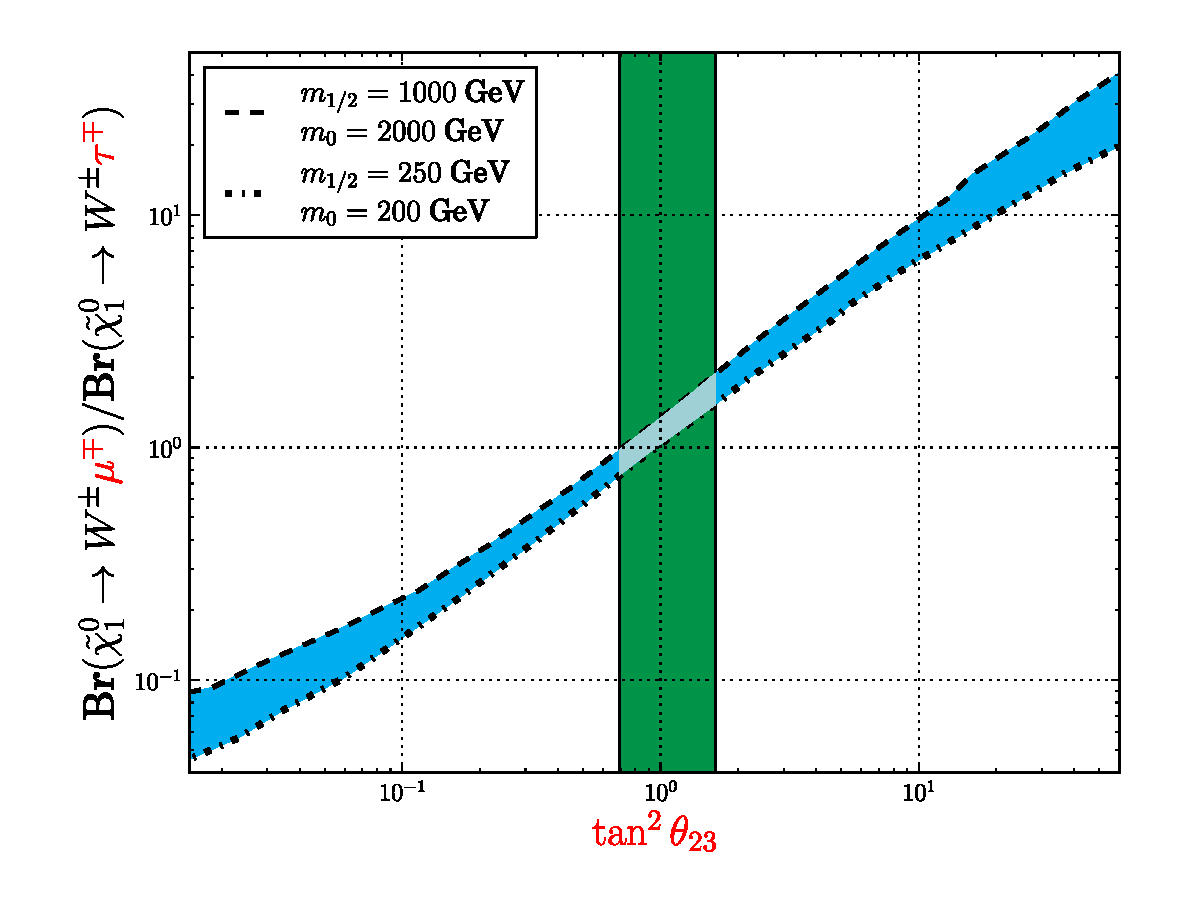
\includegraphics[scale=0.35]{atmcorrelationm}}
\put(143,20){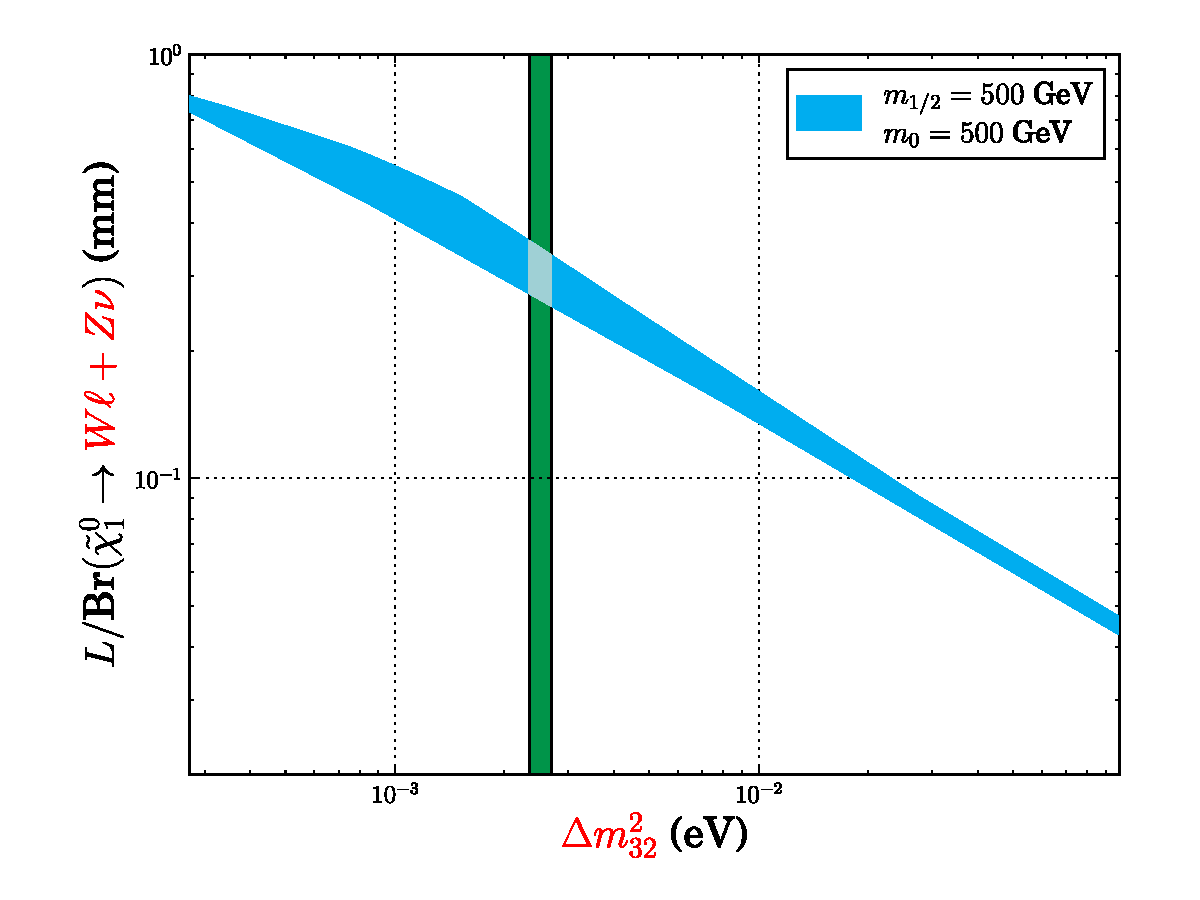
\includegraphics[scale=0.35]{LoverWlZnu_Dm23_500_500_randomm}}
\put(0,160){Only depend in \alert{$\Lambda_i$}}
\end{picture}
\end{frame}
%%%%%
Background like
%%%%%%%%%%%%%%%%%%%%%%%%
\begin{frame}[plain]
\begin{picture}(320,250)
\only<1>{\put(-30,-15){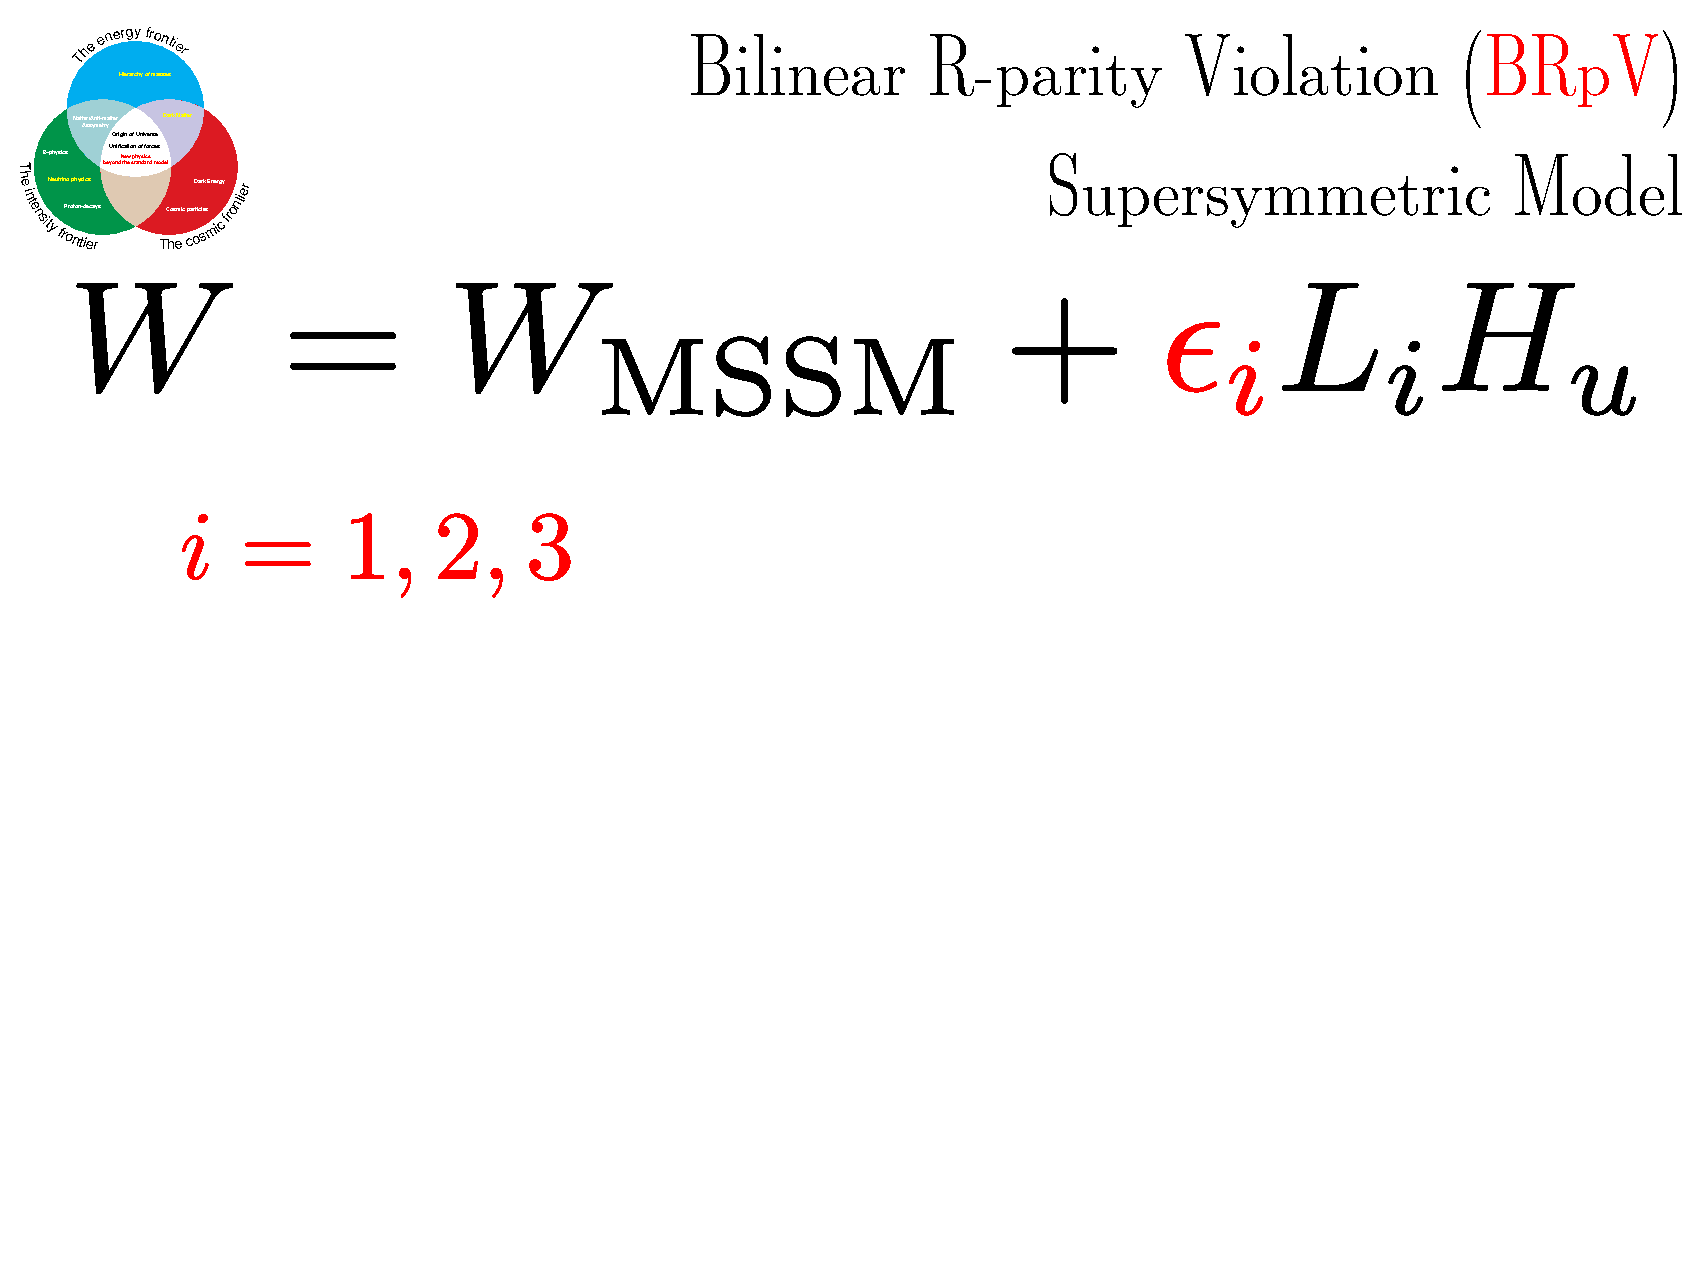
\includegraphics[width=\paperwidth]{brpv1}}}%
\only<2>{\put(-30,-15){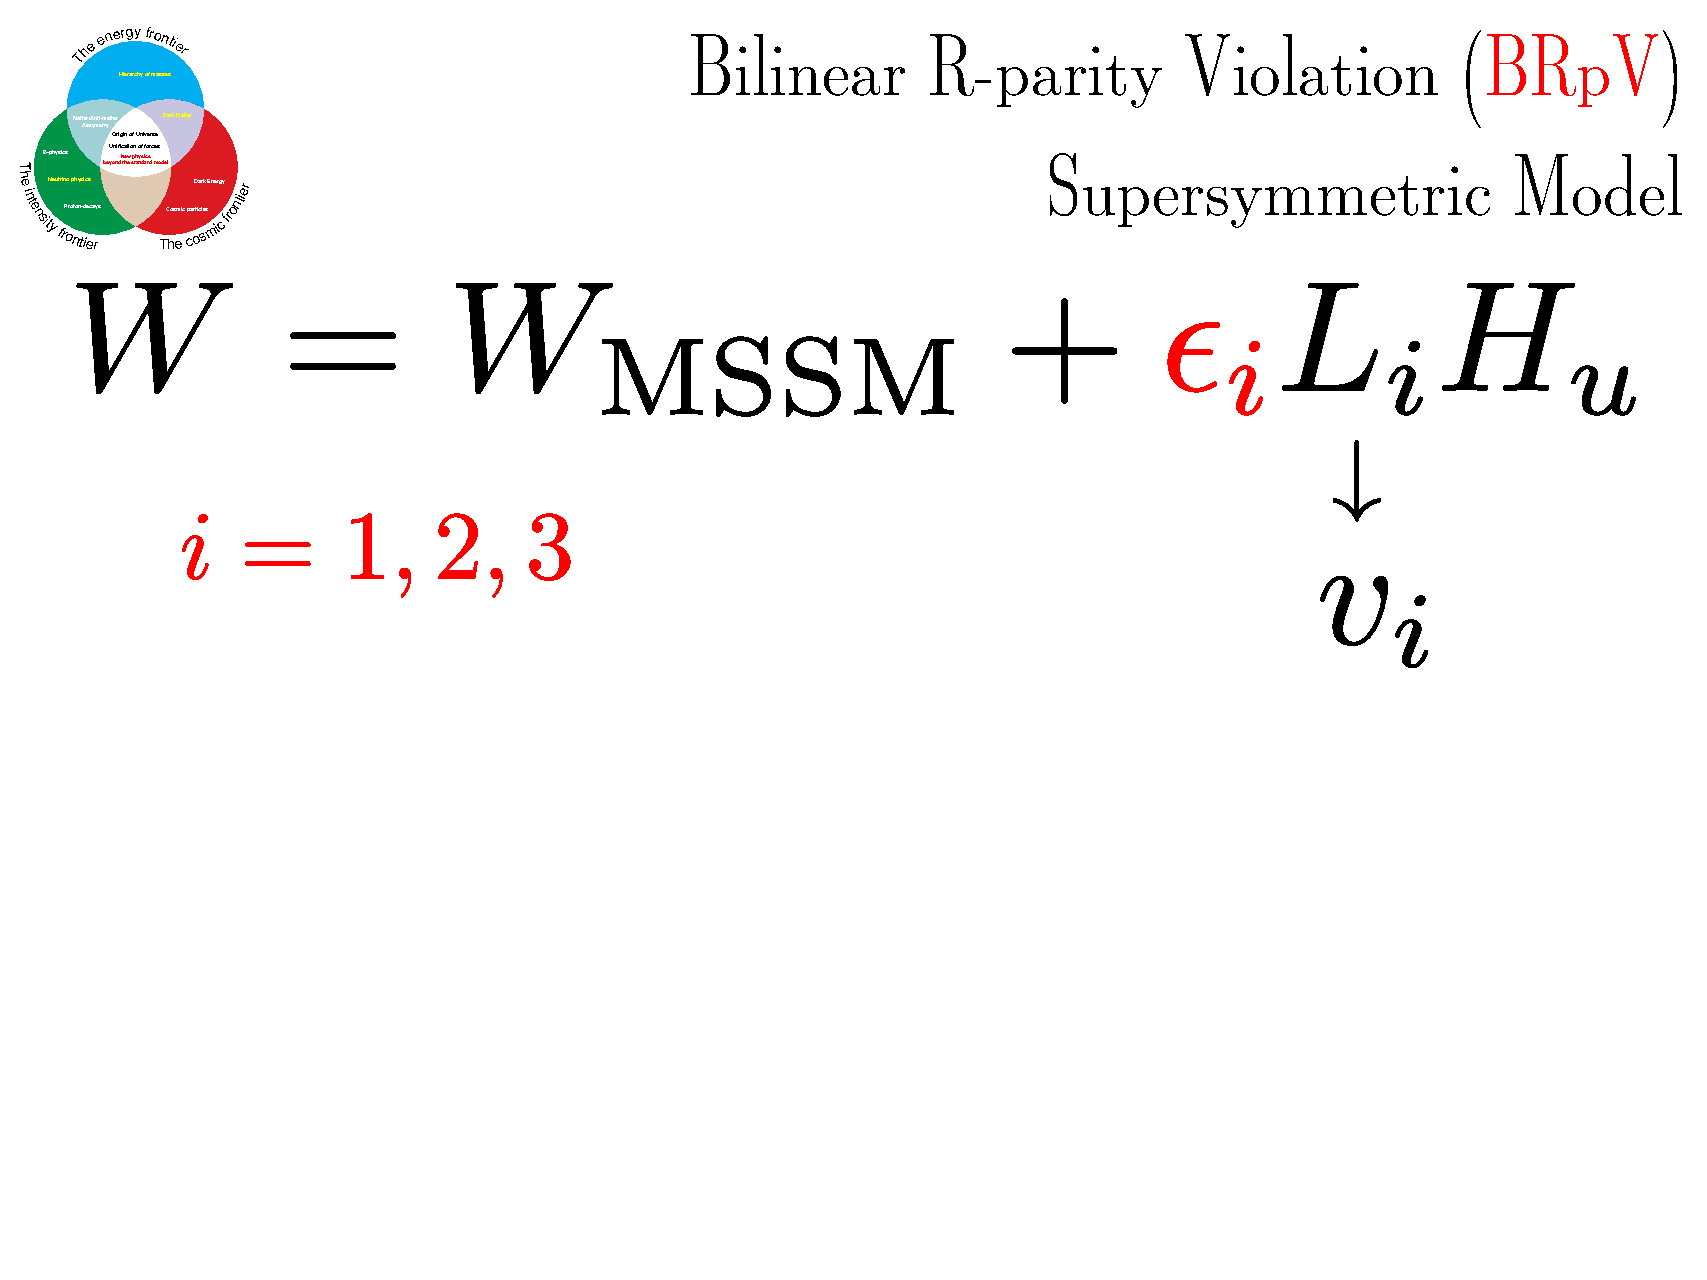
\includegraphics[width=\paperwidth]{brpv2}}}%    
\only<2>{\put(-30,-15){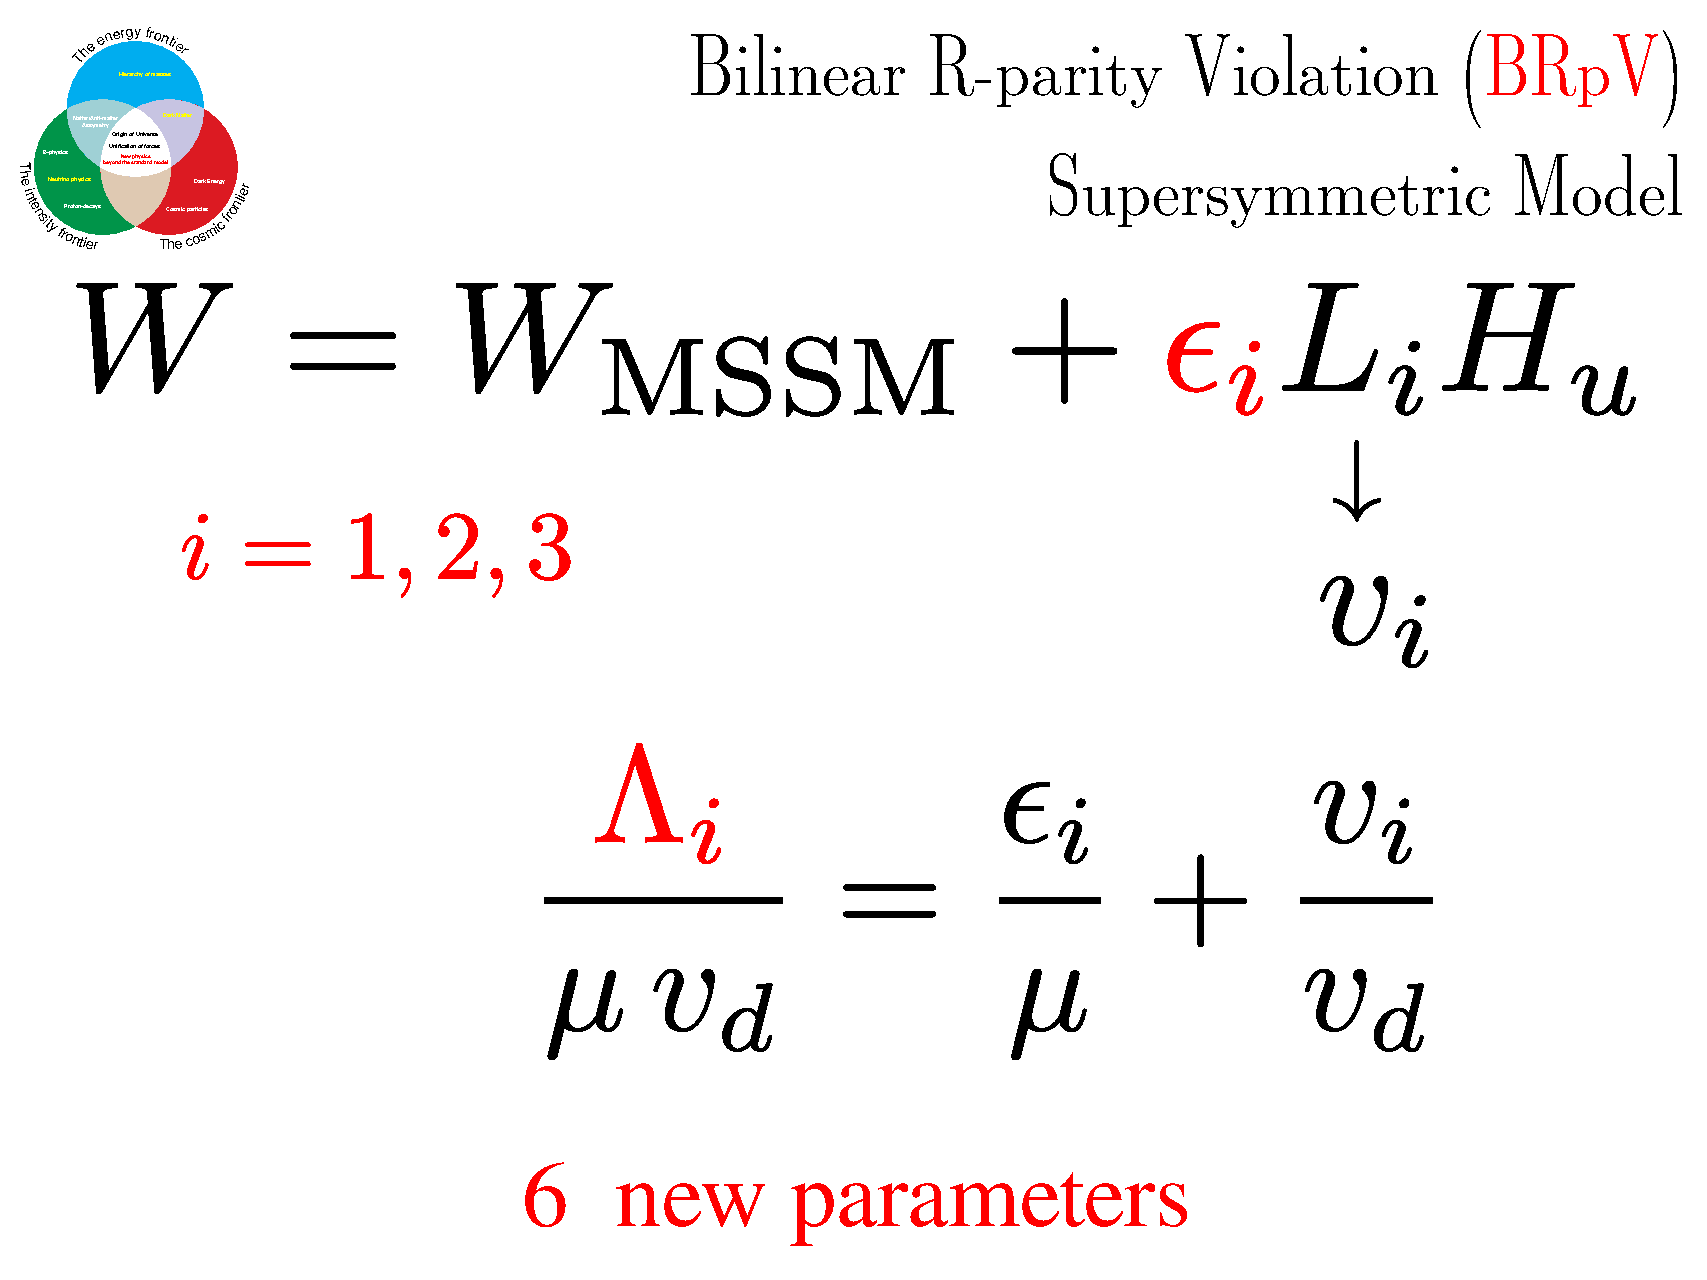
\includegraphics[width=\paperwidth]{brpv3}}}%    
\end{picture}
\end{frame}


%%%
Post it

\setbeamercolor{postit}{fg=black,bg=yellow}
\begin{beamercolorbox}[sep=1em,wd=5cm]{postit}
Place me somewhere!
\end{beamercolorbox}

%%%combine with textblock
\begin{textblock*}{297mm}(0mm,0mm)%
\begin{beamercolorbox}[sep=0.1em,wd=4cm,center,rounded=true,shadow=true]{cite}
\scriptsize Akhmedov, hep-ph/0001264
\end{beamercolorbox}
\end{textblock*}

%%More colorboxes
\setlength{\fboxrule}{3 pt}
\fcolorbox{red}{yellow}{caja de fondo
amarillo y contorno rojo}\\
\setlength{\fboxsep}{5pt}
\fcolorbox{red}{yellow}{caja de fondo
amarillo y contorno rojo}

\only<11>{\put(-20,80){
\begin{minipage}[t]{1.0\linewidth}
%\metroset{block=fill}
\begin{block}{SM particles}
     Gauge invariance+Lorentz Invariance$\to$Lagrangian (interactions)   
\end{block}
    \end{minipage}
}}


\begin{frame}
\begin{picture}(320,250)
\only<1->{\put(0,100){
  \begin{overpic}[scale=0.4,grid
            ]{table1}
\put(40,38){\tikz \draw[red,thick,rounded corners] (0,0) rectangle (2,0.5);}
  \end{overpic}
}
}
%%%circle
\end{picture}
\end{frame}

\begin{frame}[fragile]
  \frametitle{\url{./parameters.m}}
  {
    \lstset{basicstyle=\ttfamily\scriptsize,emph={g1,g2,g3,v,ThetaW,ZZ},
      emphstyle=\color{red}}
    \begin{lstlisting}[language=Mathematica]
      ...
      {g1,        { Description -> ``Hypercharge-Coupling''}},
      {g2,        { Description -> ``Left-Coupling''}},
      {g3,        { Description -> ``Strong-Coupling''}},
      ...
      {v,          { Description -> ``EW-VEV'',
          DependenceNum -> Sqrt[4*Mass[VWp]^2/(g2^2)],
          DependenceSPheno -> None  }},

      {ThetaW,    { Description -> ``Weinberg-Angle'',
          DependenceNum -> ArcSin[Sqrt[1 - Mass[VWp]^2/Mass[VZ]^2]]}},

      {ZZ, {Description -> ``Photon-Z Mixing Matrix''}},

      ...
    \end{lstlisting}
  }
  \end{frame}